\newpage
\section{Тестирование}
\setcounter{figure}{0}

Так как для данной системы не существует спроектированных УСПД и ССД для тестирования необходимо реализовать эмуляторы УСПД и ССД. 

\subsection{Эмулятор УСПД}

Для основы эмулятора УСПД был выбран одноплатный компьютер Raspberry Pi B+ под управлением операционной системы Raspbian. Для данного устройство разработана программа, которая ожидает подключения и при появлении запроса на отправку данных формирует пакет со сгенерированными данными в формате, описанном в разделе ``выходные данные'' данной пояснительной записки.

Программа реализована на языке C++ с использованием библиотек Qt. Qt Framework является основным инструментом для разработки ССД и СБД данной системы.

Сетевое взаимодействие в программах, написанных на языке C++ реализуется при помощи сокетов\cite{cpp}, в Qt для реализации данного взаимодействия используется надстройка над механизмом сокетов, облегчающая реализацию данного взаимодействия.

Данный механизм представлен такими классами как \cite{qt}:
\begin{itemize}
 \item QAbstrackSocket;
 \item QTcpSocket;
 \item QTcpServer;
 \item QUdpSocket.
\end{itemize}

Для реализации взаимодействия будут использоваться классы QTcpSocket и QTcpServer.

Так как УСПД является ведомым, оно должно ожидать подключения, для открытия порта, ожидающего подключения необходимо использовать объект QTcpServer. Прототип объекта, решающего это задачу, представлен ниже.

\begin{lstlisting}
 class TestServ : public QObject
{
    Q_OBJECT
public:
    explicit TestServ(QObject *parent = 0);
    ~TestServ();
    void initServ(const int &port);

private:
    QTcpServer *srv;

public slots:
    void newConnection();
};
\end{lstlisting}

Метод initServ предназначен для запуска сервера на определенному порту, передаваемом как аргумент метода.

Слот newConnection срабатывает при подключении к серверу и создает новый объект типа ClienSock для обмена данными с подключенным пользователем.

Прототип объекта ClienSock:

\begin{lstlisting}
 class ClientSock : public QObject
{
    Q_OBJECT
public:
    explicit ClientSock(QTcpSocket *sock, QObject *parent = 0);
    ~ClientSock();
    void sendData(QByteArray data);
    
private:
    QTcpSocket * sc;

public slots:
    QByteArray getData();
};
\end{lstlisting}

В конструкторе создается копия сокета, по которому происходит обмен данными с клиентом.

Слот getData срабатывает при получении данных от клиента. После чего запрос обрабатывается и происходит отправка ответа.

Метод sendData отправляет массив байт клиенту.

Так как данная программа только эмулирует действия УСПД, присвоим ему ID = 3, состояние УСПД представим строкой символов ``it's USPD status'', а показания УУ строкой символов ``it's UU data''.

% \subsection{Взаимодействие с УСПД}
% 
% Для сетевого взаимодействия с УСПД была создана программа с графическим итерфейсом. Задачей данной программы является установление соединения с определенным адресом и получением/отправкой текстовой информации.
% 
% Прототип объекта, решающего эту задачу, выглядит так:
% 
% \begin{lstlisting}
% class EmulSocket : public QObject
% {
%     Q_OBJECT
% public:
%     explicit EmulSocket(QObject *parent = 0);
%     ~EmulSocket();
%     void configure(QString, int);
%     void initSocket();
%     void sendData(QByteArray);
% 
% private:
%     QString qs_Address;
%     int i_Port;
%     QTcpSocket * sc;
% signals:
%     void haveData(QString);
% public slots:
%     QString getData();
% };
% \end{lstlisting}
% 
% В конструкторе и диструкторе объекта инициализируется и уничтожается объект QTcpSocket *sc.
% 
% Метод configure(QString, int) заполняет значения ip-адреса и порта назначения (поля qs\_Address и i\_Port соответственно), так же в данном методе происходит связывание события ``приняты данные'' с обработчиком этого события - методом getData(). После чего вызывается метод initSocket().
% 
% Метод initSocket() отвечает за установление соединения с указанным хостом.
% 
% Метод sendData(QByteArray) - это функция, отправляющая полученный массив байт по адресу назначения.
% 
% Сигнал haveData(QString) - это вспомогательный сигнал для взаимодействия объекта с графическим интерфейсом.
% 
% Метод getData() обрабатывает входящий поток данный и при получении данных испускает сигнал haveData(QString) в котором передает полученные данные.
% 
% Интерфейс программы представлен на рисунке \ref{window1:window1}.
% 
% \begin{figure}[h!]
%  \center{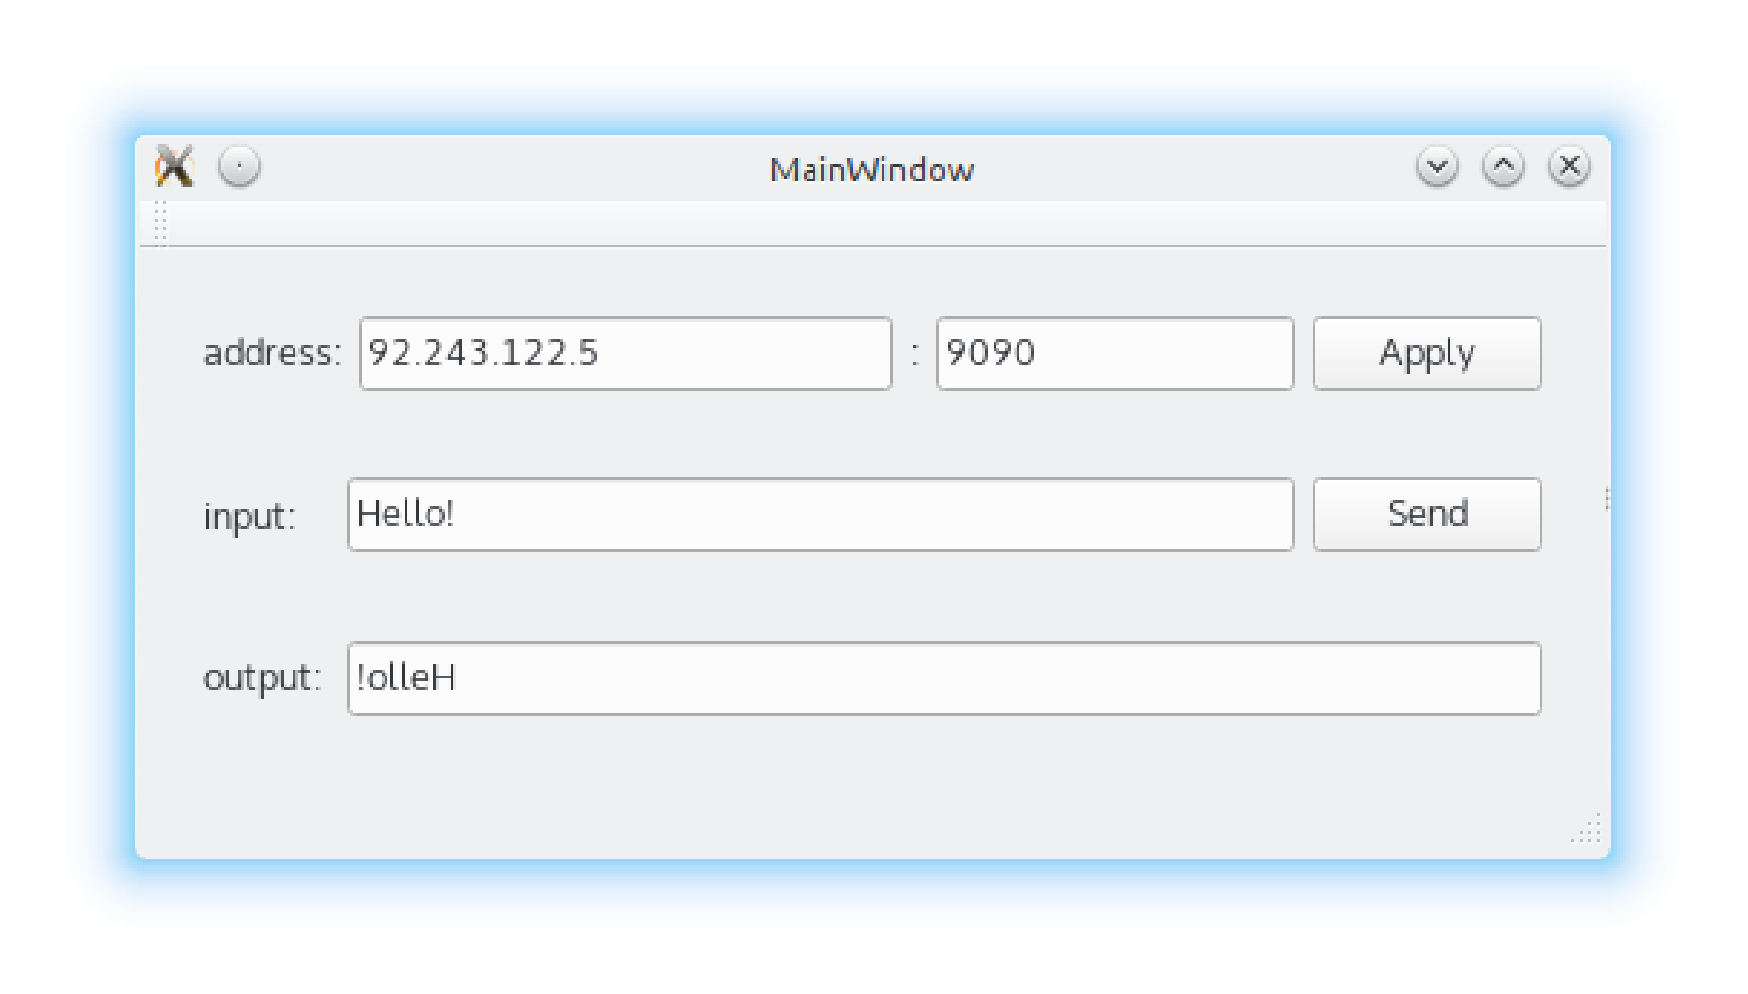
\includegraphics[width=0.8\linewidth]{window1}}
%  \caption{Подключение к эмулятору УСПД}
%  \label{window1:window1}
% \end{figure}

\subsection{Эмулятор ССД}

На сервере хранится список пользователей, которых поочередно опрашивает сервер. Данный список необходимо читать и редактировать.

Для решения данной задачи необходимо создать класс, описывающий объект-сервер, который будет хранить список клиентов и выполнять опрос клиентов.

На данный момент нет описания к системе команд УСПД, поэтому ограничимся передачей любого тестового сообщения клиенту при помощи реализованных ранее классов-сокетов.

Прототип класса-сервера представлен ниже:

\begin{lstlisting}
class MyServer : public QObject
{
    Q_OBJECT
public:
    explicit MyServer(QObject *parent = 0);
    ~MyServer();

    void addClient(const QString &name, 
		   const QString &addr, 
		   const int &port);
    QMap<QString, ClientAddress>* getClientsList();

private:
    QMap<QString, ClientAddress> clients;
    void timerEvent(QTimerEvent* event);
};
\end{lstlisting}

В конструкторе данного класса запускается таймер, которй отсчитывает интервалы времени между опросами списка клиентов. При обнулении таймера вызывается метод timerEvent в котором и происходит опрос списка клиентов, хранящегося в QMap<QString, ClientAddress>, ClientAddress - структура данных, хранящая ip-адрес и порт назначения.

Метод addClient принимает имея, ip-адрес и порт клиента, которого необходимо добавить в список и создает новый элемент в объекте clients.

getClientsList - метод, возвращающий атрибут clients.

timerEvent - метод, который просматривает список клиентов, для каждого клиента создает свое объект типа ClienSock(описан ранее), посылает клиенту массив байт, и отключается. 

Графический интерфейс программы представлен на рисунку \ref{server_gui:server_gui}.

\begin{figure}[ht!]
 \center{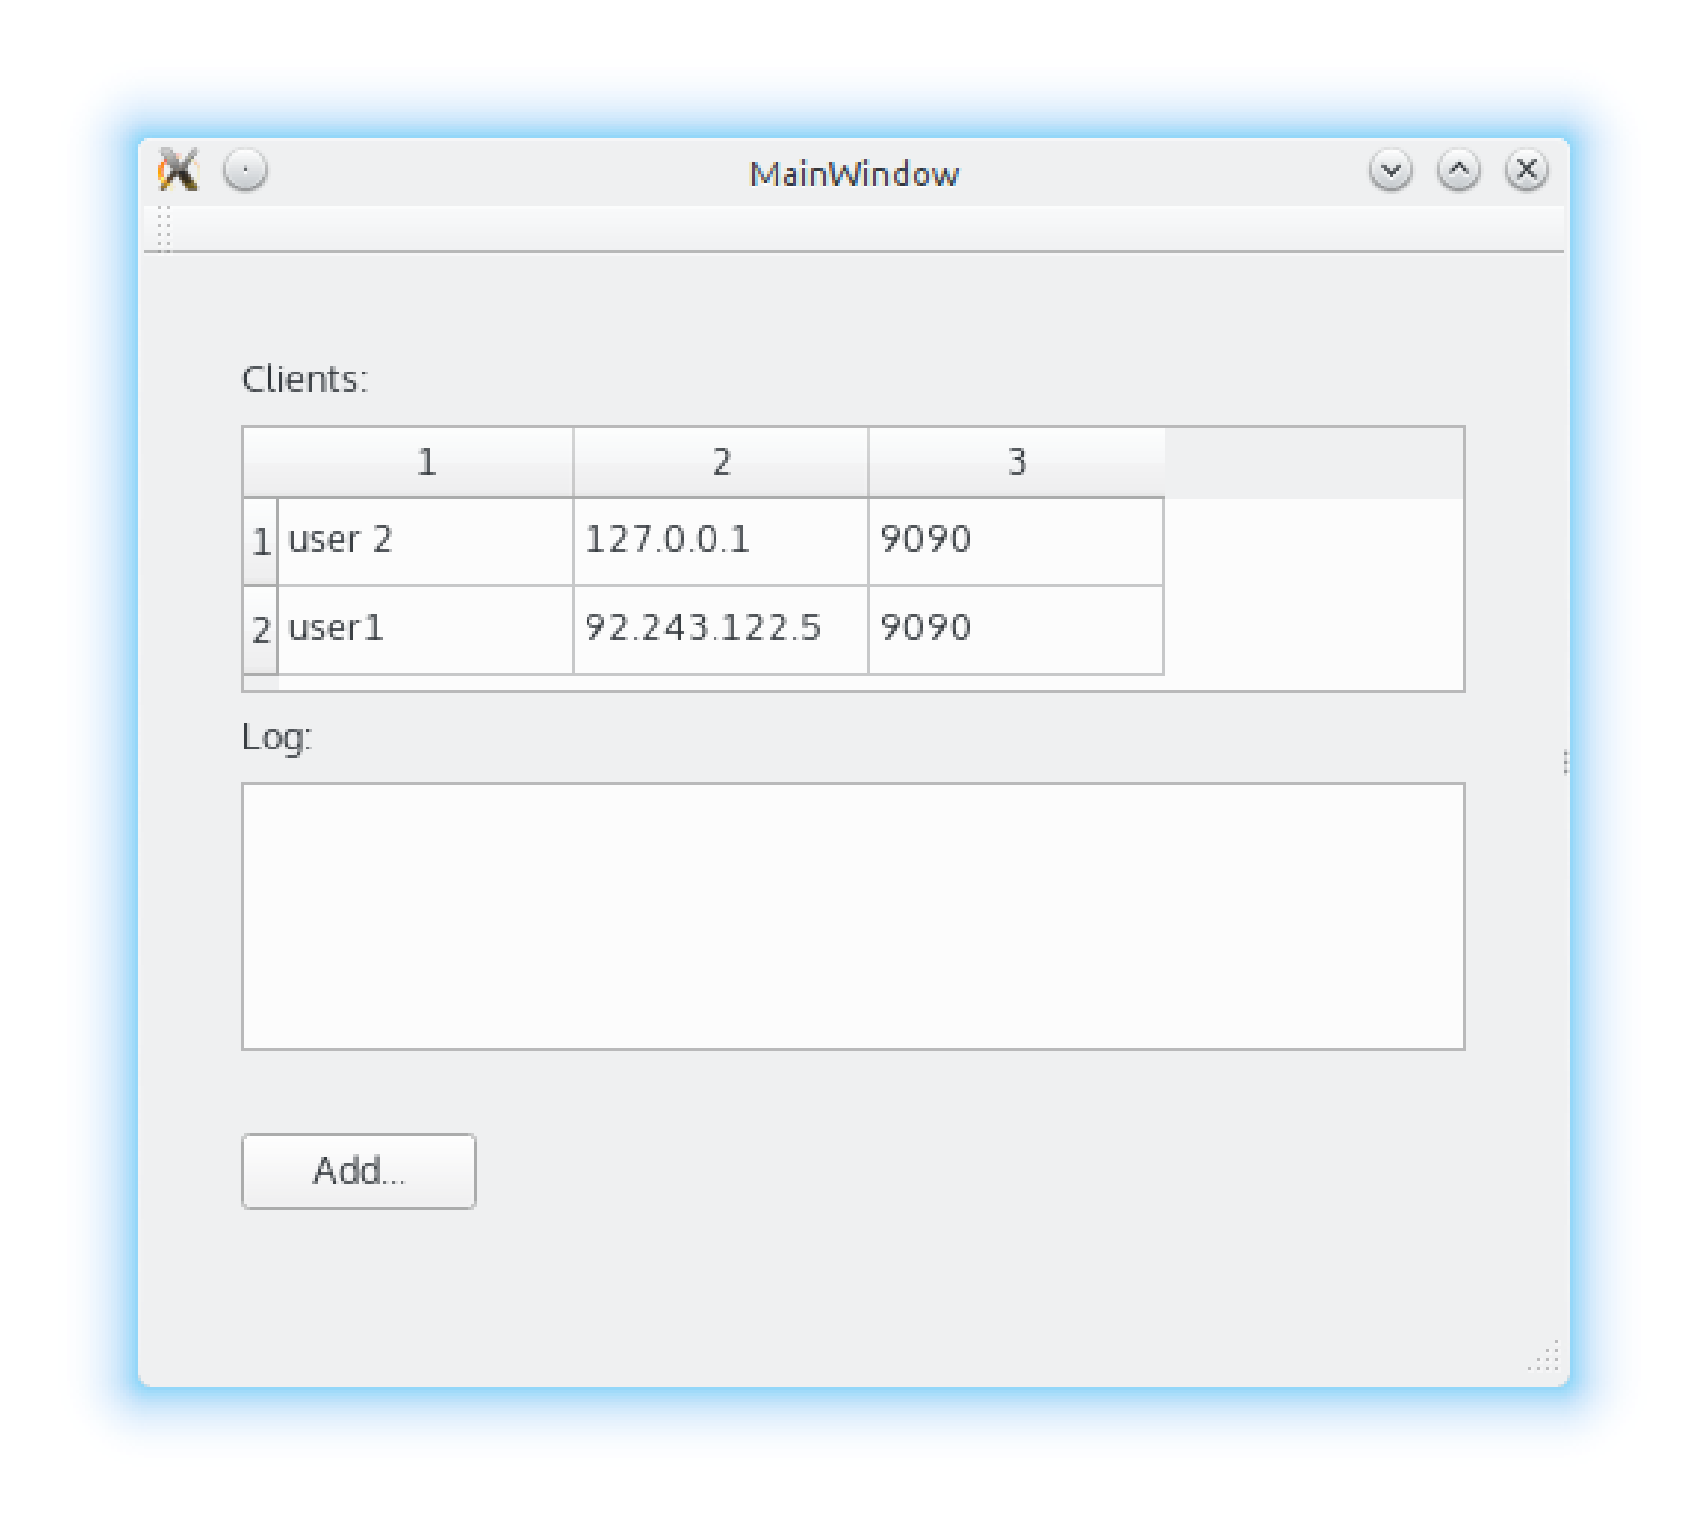
\includegraphics[width=0.7\linewidth]{server_gui}}
 \caption{Интерфейс программы}
 \label{server_gui:server_gui}
\end{figure}

Реакция эмулятора УСПД на user1 представлена на рисунке \ref{client_log:client_log}.

\begin{figure}[ht!]
 \center{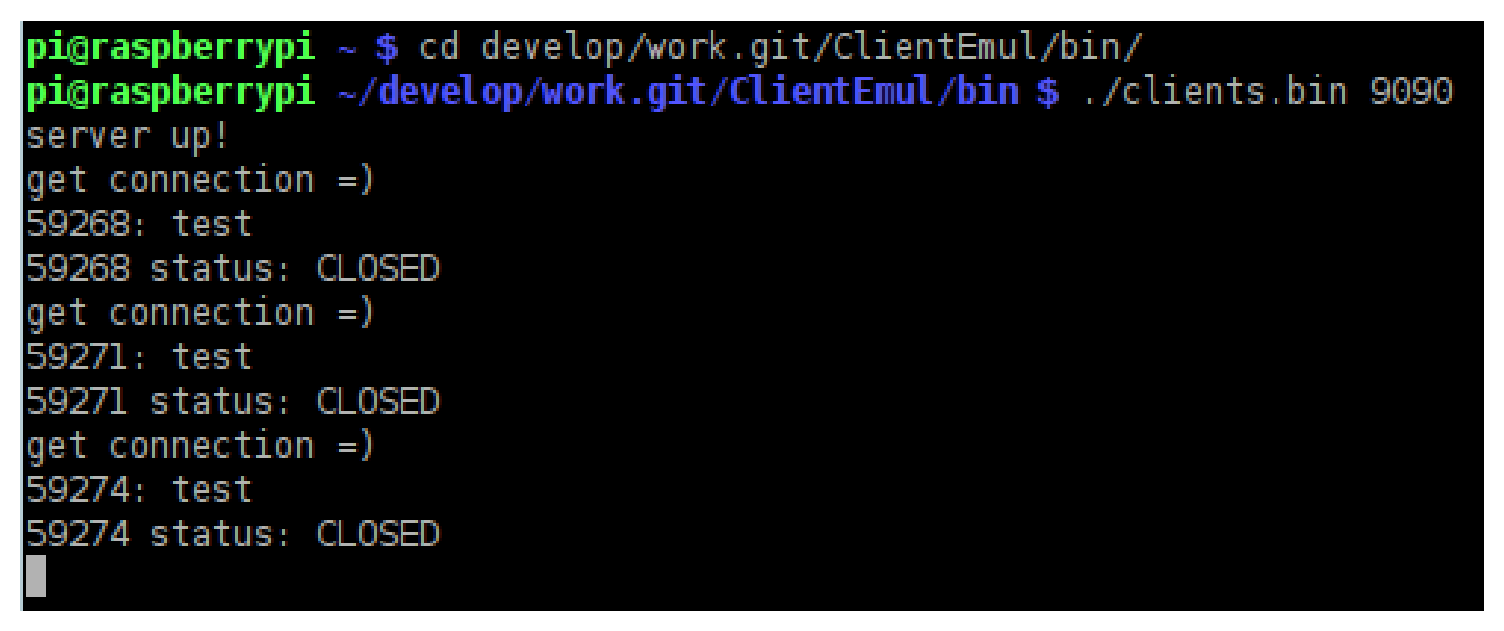
\includegraphics[width=0.7\linewidth]{client_log}}
 \caption{Работа эмулятора УСПД}
 \label{client_log:client_log}
\end{figure}

\subsection{Проверка формирования пакетов}

Для тестирования работы протокола запустим эмулятор УСПД, после чего запустим эмулятор ССД и введем адрес УСПД. Запустим wireshark\cite{nix} и дождемся очередного цикла опроса. После чего восстановим TCP сессию и рассмотрим структуру ответа. Структура ответа представлена на рисунке \ref{img:test_pachete}.

\begin{figure}[ht!]
 \center{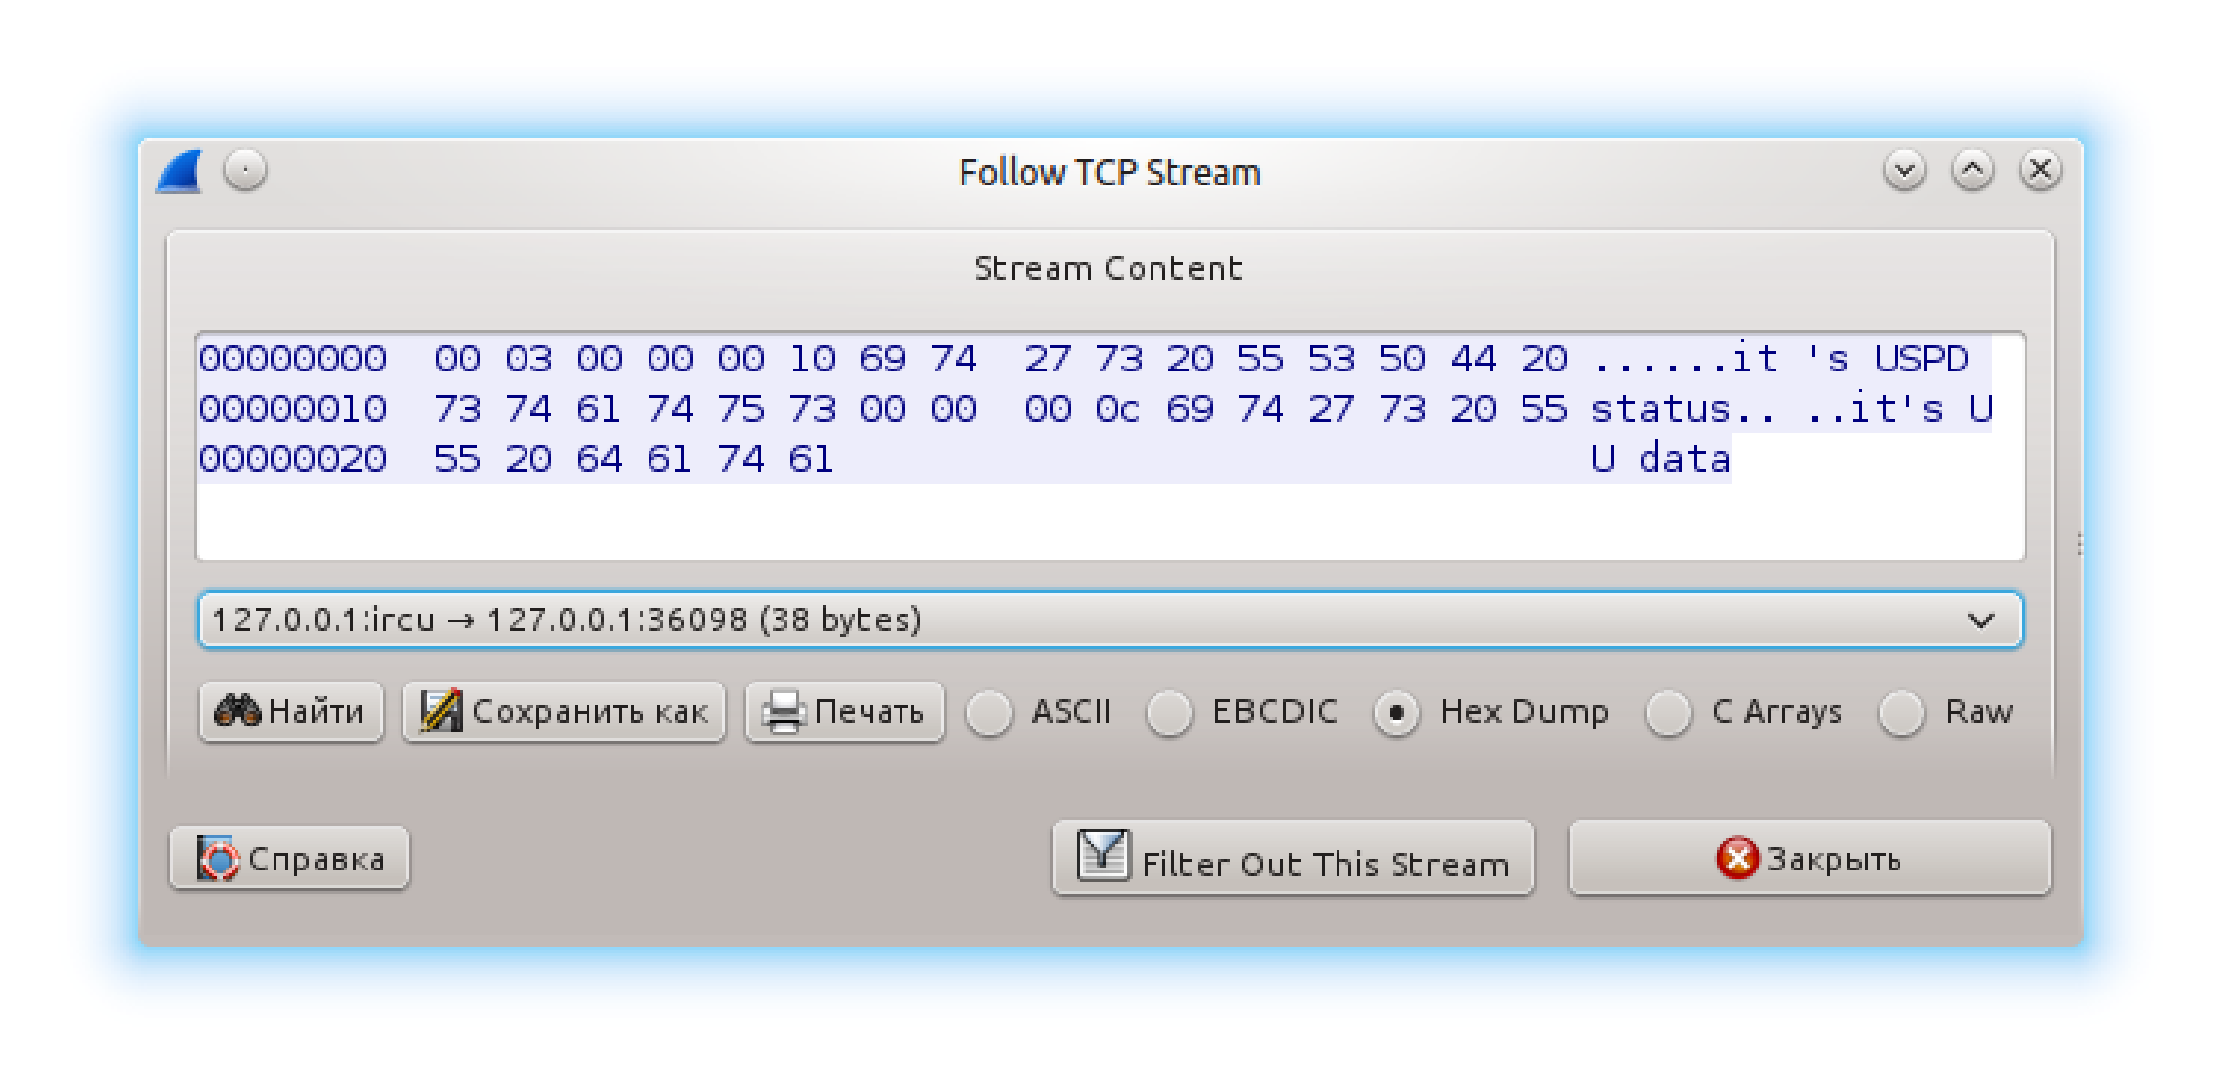
\includegraphics[width=0.7\linewidth]{test_pachete}}
 \caption{Ответ УСПД}
 \label{img:test_pachete}
\end{figure}

На рисунке представлена часть с ответом УСПД восстановленной TCP-сессии между эмуляторами. Разберем структура по байтам:

\begin{itemize}
 \item 00 03 - первые два байта, двухбайтовый ID УСПД. Совпадает с тестовыми данными УСПД;
 \item 00 00 00 10 - 4 байта - размер блока информации о состоянии УСПД. Равен 16;
 \item На рисунке видно что следующие 16 байт составляют строку состояния УСПД указанную в эмуляторе;
 \item 00 00 00 0с - 4 байта - размер блока информации от устройств учетаю Равен 12;
 \item На рисунке видно что следующие 12 байт составляют строку данных УУ указанную в эмуляторе.
\end{itemize}

На основании разбора можно сделать вывод что сформированный пакет совпадает со структурой пакета, описанной в разделе ``выходные данные''.